\makeatletter
\renewcommand*\env@matrix[1][*\c@MaxMatrixCols c]{%
  \hskip -\arraycolsep
  \let\@ifnextchar\new@ifnextchar
  \array{#1}}
\makeatother

\begin{enumerate}
%%%---part a---%%%
\item We consider the given polyhedron and the feasible basic solution
  with $x_2$ and $x_4$ in the basis. The corresponding feasible basic
  solution is
\[
x
= 
\begin{pmatrix*}[r]
0\\
1\\
0\\
2
\end{pmatrix*}
\]
and the permutation of the columns to have all basic variables first
is defined by the matrix
\[
P
=
\begin{pmatrix}[cc|cc]
0 & 0 &1 &0\\
1 & 0 &0 &0\\
0 & 0 &0 &1\\
0 & 1 &0 &0
\end{pmatrix}.
\end{equation*}
The basic direction corresponding to the non basic variable $x_1$ is
\begin{equation*}
d_1
= 
P
\begin{pmatrix*}
-B^{-1}A_1\\
1\\
0
\end{pmatrix*}
=
P
\begin{pmatrix*}
-\begin{pmatrix*}
1&0\\
1&1
\end{pmatrix*}
\begin{pmatrix*}[r]
1\\
1
\end{pmatrix*}\\
1\\
0
\end{pmatrix*}
= 
P
\begin{pmatrix*}[r]
-1\\
-2\\
1\\
0
\end{pmatrix*}
=\begin{pmatrix*}[r]
1\\
-1\\
0\\
-2
\end{pmatrix*},
\end{equation*}
and the basic direction corresponding to the non basic variable $x_3$ is
\begin{equation*}
d_3
= 
P
\begin{pmatrix*}
-B^{-1}A_3\\
0\\
1
\end{pmatrix*}
=
P
\begin{pmatrix*}
-\begin{pmatrix*}
1&0\\
1&1
\end{pmatrix*}
\begin{pmatrix*}
1\\
0
\end{pmatrix*}\\
0\\
1
\end{pmatrix*}
= 
P
\begin{pmatrix*}[r]
-1\\
-1\\
0\\
1
\end{pmatrix*}
=\begin{pmatrix*}[r]
0\\
-1\\
1\\
-1
\end{pmatrix*}.
\end{equation*}

Moving along $d_1$ with a step $\alpha \geq 0$, we obtain the point
\[
\cvect{
0\\
1\\
0\\
2} + \alpha \cvect{1\\
-1\\
0\\
-2
} = \cvect{\alpha \\ 1-\alpha \\ 0 \\ 2 -2\alpha},
\]
that is feasible for each $0 \leq \alpha \leq 1$. Therefore, the
direction is feasible. Moving along $d_3$  with a step $\alpha \geq 0$, we obtain the point
\[
\cvect{
0\\
1\\
0\\
2} + \alpha \cvect{0\\
-1\\
1\\
-1
} = \cvect{0 \\ 1 - \alpha \\ \alpha \\ 2-\alpha}
\]
that is feasible for each $0 \leq \alpha \leq 1$. Therefore, the
direction is also feasible.

These two directions are shown in the following figure at point
$(0,1)$, where their length corresponds to $\alpha=1$.

\begin{center}
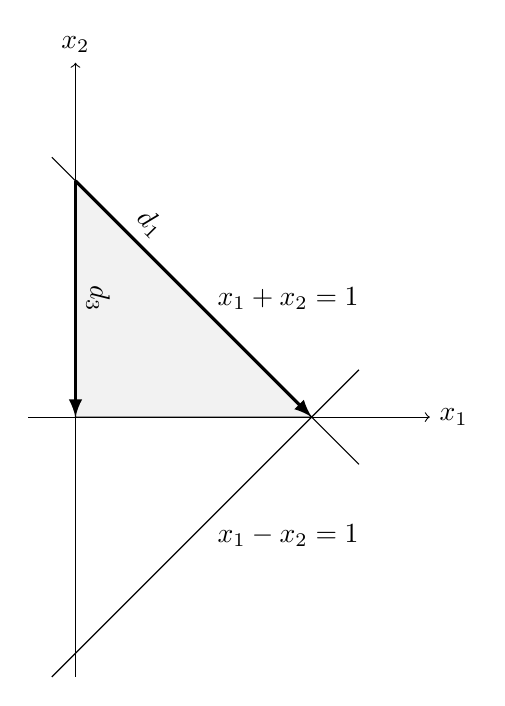
\begin{tikzpicture}[scale=3]
\draw[fill=lightgray!20]  (0,1) -- (1,0) -- (0,0) -- cycle;
\draw[->] (-0.2,0) -- (1.5,0) node[right] {$x_1$};
\draw[->] (0,-1.1) -- (0,1.5) node[above] {$x_2$};
\draw[-latex,very thick] (0,1)-- ++(1,-1) node [pos=0.25,above,sloped] {$d_1$};
\draw[-latex,very thick] (0,1)-- ++(0,-1) node [pos=0.5,above,sloped] {$d_3$}; 
\draw (-0.1,-1.1) -- (1.2,0.2);
\draw (-0.1,1.1) -- (1.2,-0.2);
\node at (0.9,0.5) {$x_1+x_2=1$};
\node at (0.9,-0.5) {$x_1-x_2=1$};
\end{tikzpicture}
\end{center}
%
%
%

%%%---part b---%%%
\item We now consider the feasible basic solution where $x_1$ and
  $x_4$ are in the basis. The feasible basic solution is
\[
x
= 
\begin{pmatrix}
1\\
0\\
0\\
0
\end{pmatrix}
\]
and the permutation matrix is
\[
P
=
\begin{pmatrix}[cc|cc]
1 & 0 &0 &0\\
0 & 0 &1 &0\\
0 & 0 &0 &1\\
0 & 1 &0 &0
\end{pmatrix}.
\]
The basic direction corresponding to the non basic variable $x_2$ is 
\begin{equation*}
\tilde{d_2}
= 
P
\begin{pmatrix*}
-B^{-1}A_2\\
1\\
0
\end{pmatrix*}
=
P
\begin{pmatrix*}
-\begin{pmatrix*}
1&0\\
-1&1
\end{pmatrix*}
\begin{pmatrix*}
1\\
-1
\end{pmatrix*}\\
1\\
0
\end{pmatrix*}
= 
P
\begin{pmatrix*}[r]
-1\\
2\\
1\\
0
\end{pmatrix*}
=\begin{pmatrix*}[r]
-1\\
1\\
0\\
2
\end{pmatrix*},
\end{equation*}
and the basic direction corresponding to the non basic variable $x_3$ is
\begin{equation*}
\tilde{d_3} = 
P \begin{pmatrix*}
-B^{-1}A_3\\
0\\
1
\end{pmatrix*}
= P
\begin{pmatrix*}
-\begin{pmatrix*}
1&0\\
-1&1
\end{pmatrix*}
\begin{pmatrix*}
1\\
0
\end{pmatrix*}\\
0\\
1
\end{pmatrix*}
= 
P
\begin{pmatrix*}[r]
-1\\
1\\
0\\
1
\end{pmatrix*}
=\begin{pmatrix*}[r]
-1\\
0\\
1\\
1
\end{pmatrix*}.
\end{equation*}

Moving along $\tilde{d}_2$ with a step $\alpha \geq 0$, we obtain the point
\[
\cvect{
1\\
0\\
0\\
0} + \alpha \cvect{-1\\
1\\
0\\
2
} = \cvect{1 - \alpha \\ \alpha \\ 0 \\ 2\alpha},
\]
that is feasible for any $0 \leq \alpha \leq 1$. Therefore, the
direction is feasible.
Moving along $\tilde{d}_3$ with a step $\alpha \geq 0$, we obtain the point
\[
\cvect{
1\\
0\\
0\\
0} + \alpha \cvect{-1\\
0\\
1\\
1
} = \cvect{1-\alpha \\ 0 \\ \alpha \\ \alpha},
\]
that is feasible for any $0 \leq \alpha \leq 1$. Therefore, the
direction is feasible.
These two directions are shown in the following figure at point
$(1,0)$, where their length corresponds to $\alpha=1$.

\begin{center}
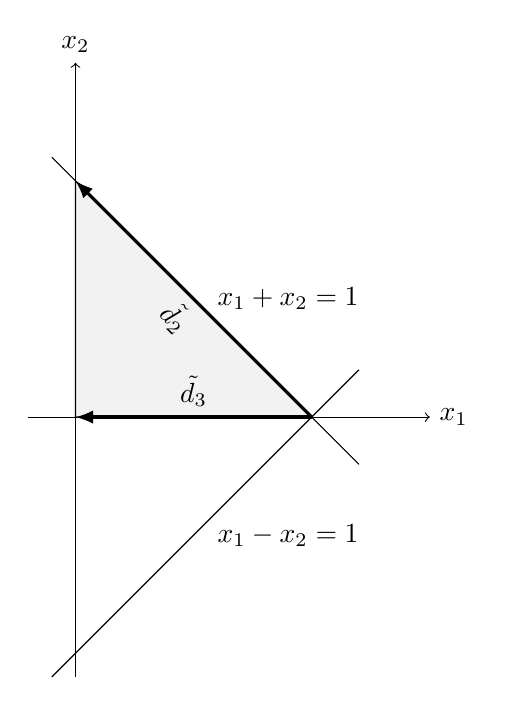
\begin{tikzpicture}[scale=3]
\draw[fill=lightgray!20]  (0,1) -- (1,0) -- (0,0) -- cycle;
\draw[->] (-0.2,0) -- (1.5,0) node[right] {$x_1$};
\draw[->] (0,-1.1) -- (0,1.5) node[above] {$x_2$};
\draw[-latex,very thick] (1,0)-- ++(-1,1) node[pos=0.5,below,sloped] {$\tilde{d_2}$};
\draw[-latex,very thick] (1,0)-- ++(-1,0) node[pos=0.5,above,sloped] {$\tilde{d_3}$};
\draw (-0.1,-1.1) -- (1.2,0.2);
\draw (-0.1,1.1) -- (1.2,-0.2);
\node at (0.9,0.5) {$x_1+x_2=1$};
\node at (0.9,-0.5) {$x_1-x_2=1$};
\end{tikzpicture}
\end{center}

%
%
%
%%%---part c---%%%
\item Finally, consider the feasible basic solution where $x_1$ and $x_2$ are in the basis. Then,
\begin{equation*}
x = 
\begin{pmatrix*}[r]
1\\
0\\
0\\
0
\end{pmatrix*}
\text{ and } P
=
\begin{pmatrix}[cc|cc]
1 & 0 &0 &0\\
0 & 1 &0 &0\\
0 & 0 &1 &0\\
0 & 0 &0 &1
\end{pmatrix}
=
I.
\end{equation*}
The basic direction corresponding to the non basic variable $x_3$ is
\begin{equation*}
\hat{d_3} = 
\begin{pmatrix*}
-B^{-1}A_3\\
1\\
0
\end{pmatrix*}
=
\begin{pmatrix*}
-\begin{pmatrix*}
\frac{1}{2}&\frac{1}{2}\\
\frac{1}{2}&-\frac{1}{2}
\end{pmatrix*}
\begin{pmatrix*}
1\\
0
\end{pmatrix*}\\
1\\
0
\end{pmatrix*}
= 
\begin{pmatrix*}[r]
-\frac{1}{2}\\
-\frac{1}{2}\\
1\\
0
\end{pmatrix*},
\end{equation*}
and the basic direction corresponding to the non basic variable $x_4$ is
\begin{equation*}
\hat{d_4} = 
\begin{pmatrix*}
-B^{-1}A_4\\
0\\
1
\end{pmatrix*}
=
\begin{pmatrix*}
-\begin{pmatrix*}
\frac{1}{2}&\frac{1}{2}\\
\frac{1}{2}&-\frac{1}{2}
\end{pmatrix*}
\begin{pmatrix*}
0\\
1
\end{pmatrix*}\\
1\\
0
\end{pmatrix*}
= 
\begin{pmatrix*}[r]
-\frac{1}{2}\\
\frac{1}{2}\\
0\\
1
\end{pmatrix*}.
\end{equation*}
Moving along $\hat{d}_3$ with a step $\alpha \geq 0$, we obtain the point
\[
\cvect{
1\\
0\\
0\\
0} + \alpha \cvect{-\frac{1}{2}\\
-\frac{1}{2}\\
1\\
0
} = \cvect{1 - \frac{1}{2}\alpha \\ -\frac{1}{2}\alpha \\ \alpha \\ 0},
\]
that is not feasible for any $\alpha > 0$ as the second entry is negative. Therefore, the
direction is \textbf{not} feasible.

Moving along $\hat{d}_4$ with a step $\alpha \geq 0$, we obtain the point
\[
\cvect{
1\\
0\\
0\\
0} + \alpha \cvect{-\frac{1}{2}\\
\frac{1}{2}\\
0\\
1
} = \cvect{1 -  \frac{1}{2} \alpha \\ \frac{1}{2} \alpha \\ 0 \\ \alpha},
\]
that is feasible for any $0 \leq \alpha \leq 2$. Therefore, the
direction is feasible.


These two directions are shown in the following figure at point
$(1,0)$, where their length corresponds to $\alpha=1$. Note that $\hat{d_4}$ is a feasible direction, whereas $\hat{d_3}$ is not.

\begin{center}
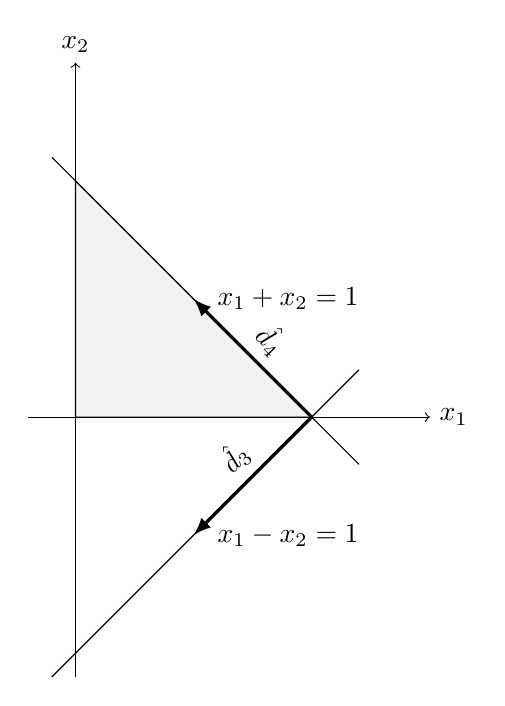
\begin{tikzpicture}[scale=3]
\draw[fill=lightgray!20]  (0,1) -- (1,0) -- (0,0) -- cycle;
\draw[->] (-0.2,0) -- (1.5,0) node[right] {$x_1$};
\draw[->] (0,-1.1) -- (0,1.5) node[above] {$x_2$};
\draw[-latex,very thick] (1,0)-- ++(-0.5,-0.5) node[pos=0.5,above,sloped] {$\hat{d_3}$};
\draw[-latex,very thick] (1,0)-- ++(-0.5,0.5) node[pos=0.5,above,sloped] {$\hat{d_4}$};
\draw (-0.1,-1.1) -- (1.2,0.2);
\draw (-0.1,1.1) -- (1.2,-0.2);
\node at (0.9,0.5) {$x_1+x_2=1$};
\node at (0.9,-0.5) {$x_1-x_2=1$};
\end{tikzpicture}
\end{center}

\end{enumerate}

